% Author: Mabel Delgado

\documentclass[18pt]{beamer}

% To accept special characters from the keyboard
\usepackage[utf8]{inputenc}
% To altere the language of the document
\usepackage[spanish]{babel}
% To include figures
\usepackage{graphicx}
% To write mathematical formulation
\usepackage{amsmath}
% To include special fonts in mathematical formulation
\usepackage{amsfonts}
% To include special symbols in the mathematical formulation
\usepackage{amssymb}
% To include links in the references
\usepackage{url}
% To use colors
\usepackage{xcolor}
% To use hyperreferences
\usepackage{hyperref}
% To display code snippets
\usepackage{listings}

% Hyperlinks colors customization
\hypersetup{
	colorlinks = true,
  	urlcolor = blue,
  	citecolor = blue,
  	linkcolor = white  
}

% Define a new footnote object (without marker/associated number)
\newcommand\blfootnote[1]{%
  \begingroup
  \renewcommand\thefootnote{}\footnote{#1}%
  \addtocounter{footnote}{-1}%
  \endgroup
}

% Use python as code
\lstset{basicstyle=\ttfamily,
		language=python,
		showstringspaces=false}

% Remove figure word from figures
\setbeamertemplate{caption}{\raggedright\insertcaption\par}

% Remove navigation symbols
\setbeamertemplate{navigation symbols}{}

% Theme
\usetheme{Copenhagen}

% Information to be included in the title page
\title{¿Qué es la comunidad Python?}
\author{Mabel Delgado (@mabeldelgadob)}
\institute{AI Saturdays (Almería)}
\date{16 de marzo de 2019}

\begin{document}

% TITLE
\begin{frame}
	\titlepage
\end{frame}

% SOBRE MÍ
\begin{frame}
	\frametitle{Un poco sobre mí...}
	\begin{columns}
		\column{.35\textwidth}
		\centering
			
\includegraphics[width=2.5cm]{images/aeropython.png}\\
			
\includegraphics[width=3.5cm]{images/pyladiesmadrid_alargado.png}\\
			
\includegraphics[width=1.5cm]{images/python_spain.png}
			
\includegraphics[width=1.5cm]{images/django_girls.jpg}\\
			
\includegraphics[width=3.5cm]{images/psf.png}
				
		\column{.65\textwidth}
		\begin{itemize}
			\setlength\itemsep{0.6em}		
			\item Ingeniera aeronáutica (UPM).
			\item Métodos y herramientas  ensayos en vuelo de aviones.
			\item Miembro AeroPython.
			\item Co-Fundadora PyLadies Madrid.
			\item Vocal Asociación Python España.
			\item Co-organizadora eventos Django Girls (Cáceres, Palma, Málaga).
			\item Fellow Member Python Software Foundation.
		\end{itemize}		
	\end{columns}
\end{frame}


% PYTHON INTRO
\begin{frame}

	\frametitle{¿Qué es Python?}
	\begin{columns}
		\column{.35\textwidth}
		\centering
			
\includegraphics[width=2.5cm]{images/python_logo_cuadrado.png}
			
		\column{.65\textwidth}
		\begin{itemize}
			\setlength\itemsep{0.6em}		
			\item Lenguaje de programación creado por Guido van Rossum en 1991.
			\item Libre y gratuito.
			\item Interpretado y tipado dinámico.
			\item De alto nivel y de propósito general.
			\item Gestión automática de memoria.
			\item Múltiples paradigmas de programación (OOP, Funcional...).
			\item Multitud de paquetes para realizar diferentes tareas.
		\end{itemize}
	\end{columns}
	
\end{frame}


% PYTHON ANTIGRAVITY
\begin{frame}

	\frametitle{Oh yeah, Python!!!}
	
	$>>>$ import antigravity
    
	\begin{figure}
		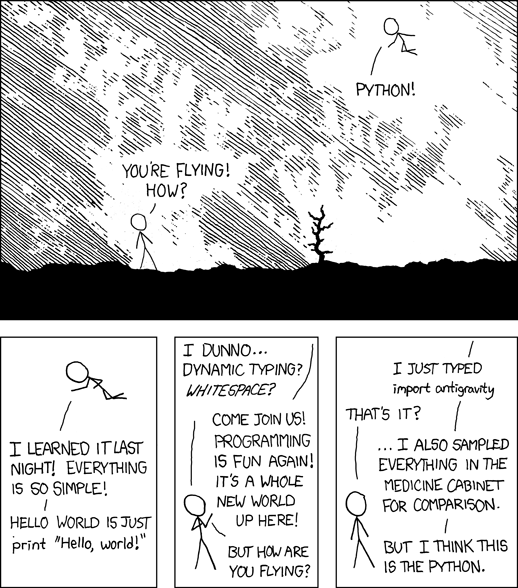
\includegraphics[width=5.5cm]{images/xkcd.png}
	\end{figure}
	
	\blfootnote{\scriptsize https://xkcd.com/353/}
	
	
\end{frame}


% PYTHON COMMUNITY
\begin{frame}

	\frametitle{Pero Python no es sólo el lenguaje...}
	   
	\begin{figure}
		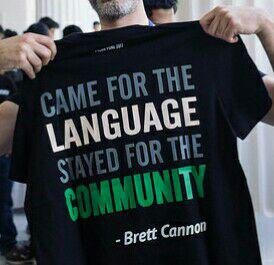
\includegraphics[width=6cm]{images/tshirt_quote.jpg}
	\end{figure}	
	
\end{frame}


% PYTHON SOFTWARE FOUNDATION
\begin{frame}

	\frametitle{Python Software Foundation (PSF)}
	
	\begin{figure}
		
\includegraphics[width=5cm]{images/psf.png}
	\end{figure}
	
	The mission of the Python Software Foundation is to promote, protect, 
	and advance the Python programming language, and to support and 
	facilitate the growth of a diverse and international 
	community of Python programmers.

    \rightline{—from the Mission Statement page}

	\vspace{0.6cm}    
	\centerline{https://www.python.org/psf/}
	
	\vspace{0.4cm}
	\centerline{@ThePSF}
	
\end{frame}


% PYTHON SOFTWARE FOUNDATION (II)
\begin{frame}

	\frametitle{Python Software Foundation (PSF) - Información}
		
	\begin{columns}
		\column{.35\textwidth}
		\centering
			
\includegraphics[width=3.5cm]{images/psf.png}
			
		\column{.65\textwidth}
		\begin{itemize}
			\setlength\itemsep{0.6em}		
			\item Organización sin ánimo de lucro (decisiones Board of Directors).
			\item Propiedad intelectual lenguaje de programación Python (licencia, trademarks).
			\item Apoya conferencias y organizaciones de Python a nivel global.
			\item Apoya económicamente proyectos de desarrollo de Python (grants program).
			\item Niveles de socios: Basic members, supporting members, managing members, 
			contributing members, fellow members.  
		\end{itemize}
	\end{columns}
	
\end{frame}


% ORGANIZACIONES NACIONALES Y LOCALES
\begin{frame}

	\frametitle{Organizaciones de Python Nacionales y Locales}
	
	\begin{figure}
		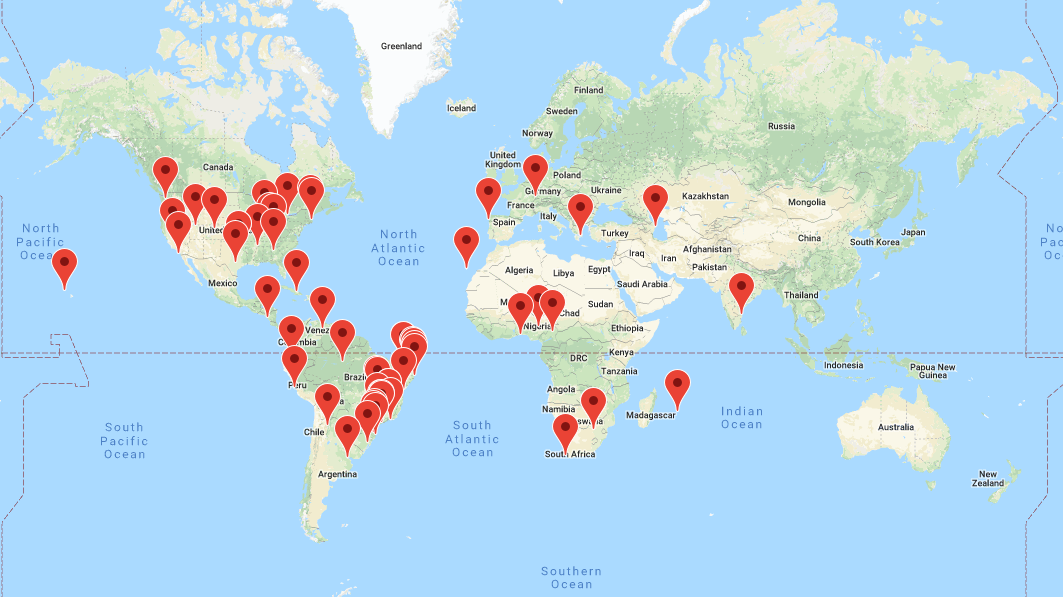
\includegraphics[width=10.5cm]{images/local_communities.png}
	\end{figure}
	
	\blfootnote{\scriptsize https://community.python.org.br/}
	
\end{frame}


% ASOCIACIÓN PYTHON ESPAÑA
\begin{frame}

	\frametitle{Asociación Python España}
	
	\begin{figure}
		
\includegraphics[width=2.5cm]{images/python_spain.png}
	\end{figure}
	
	La asociación Python España es una asociación sin ánimo de lucro cuyo propósito 
	es promover el uso del lenguaje de programación Python en España, servir como 
	punto de encuentro a aquellos interesados en su uso, y darles soporte en la medida 
	de sus posibilidades.

	\vspace{0.3cm}
	\centerline{https://www.es.python.org/}
	
	\vspace{0.4cm}
	\centerline{@python\_es}	
	
\end{frame}


% ASOCIACIÓN PYTHON ESPAÑA (II)
\begin{frame}

	\frametitle{Asociación Python España - Información}
		
	\begin{columns}
		\column{.35\textwidth}
		\centering
			
\includegraphics[width=2.5cm]{images/python_spain.png}
			
		\column{.65\textwidth}
		\begin{itemize}
			\setlength\itemsep{0.6em}		
			\item Organización sin ánimo de lucro.
			\item Decisiones Junta de la Asociacion (renovación cada dos años).
			\item Apoya organización del congreso nacional de Python (PyConES).
			\item Soporte y ayuda financiera organizaciones locales de Python.
			\item Ser socio, ser miembro.
			\item Novedades; grupos de trabajo, discourse, pycena, 
			beneficios socios...  
		\end{itemize}
	\end{columns}
	
\end{frame}


% COMUNIDADES LOCALES PYTHON ESPAÑA
\begin{frame}

	\frametitle{Comunidades locales de Python en España}
	
	\begin{figure}
		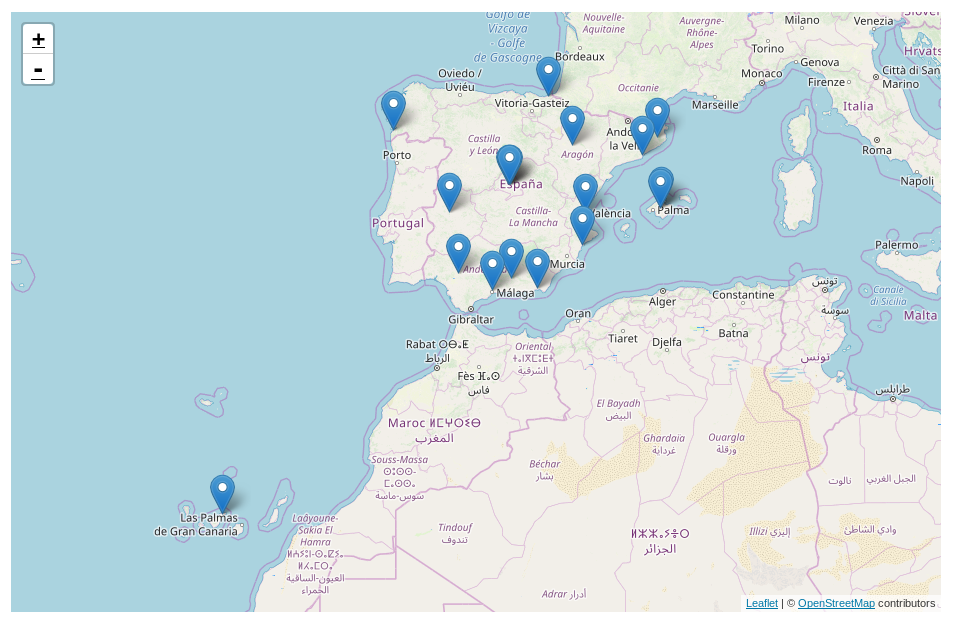
\includegraphics[width=9.5cm]{images/comunidades_locales.png}
	\end{figure}

	\centerline{Python Almería: https://www.meetup.com/Python-Almeria/}		
	
	\blfootnote{\scriptsize https://es.python.org/pages/comunidades.html}
	
\end{frame}


% COMUNIDAD DIVERSA
\begin{frame}

	\frametitle{Comunidad de Python diversa}
	
	Evolución de las mujeres en informática...
	
	\begin{figure}
		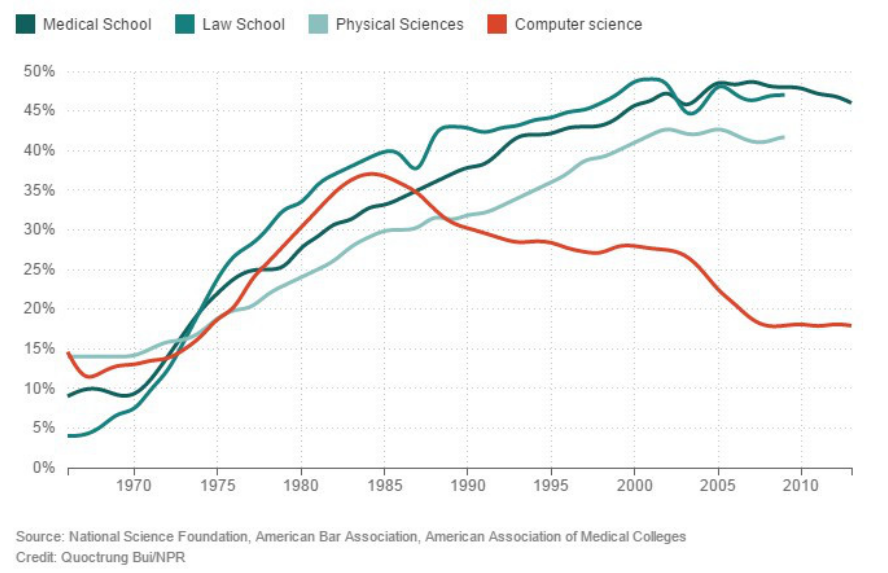
\includegraphics[width=10.5cm]{images/women_computer_science.png}
	\end{figure}
		
\end{frame}


% PYLADIES
\begin{frame}

	\frametitle{PyLadies}
	
	\begin{figure}
		
\includegraphics[width=2.5cm]{images/pyladies_cuadrado.png}
		
\includegraphics[width=5cm]{images/pyladies_alargado.png}
	\end{figure}
	
	PyLadies is an international mentorship group with a focus on helping more 
	women become active participants and leaders in the Python 
	open-source community. 
	

	\vspace{0.6cm}    
	\centerline{https://www.pyladies.com/}
	
	\vspace{0.4cm}
	\centerline{@pyladies}
	
\end{frame}


% PYLADIES - INFORMACIÓN
\begin{frame}

	\frametitle{PyLadies - Información}
		
	\begin{columns}
		\column{.35\textwidth}
		\centering
			
\includegraphics[width=2.5cm]{images/pyladies_cuadrado.png}\\
			
\includegraphics[width=3cm]{images/pyladies_alargado.png}\\
			\vspace{0.5cm}			
			\small$>>>$pip install pyladies
			
		\column{.65\textwidth}
		\begin{itemize}
			\setlength\itemsep{0.6em}		
			\item Organización sin ánimo de lucro creada en Los Ángeles en 2011.
			\item Promover, educar y avanzar en la diversidad de la comunidad de Python.
			\item Realizar cursos, conferencias, eventos y reuniones. 
			\item Crear una red de mujeres programadoras, y ponerla en contacto con el 
			resto de comunidades Python nacionales e internacionales.
			\item Cualquier persona con interés en Python está invitada a participar.  
		\end{itemize}
	\end{columns}
	
\end{frame}


% PYLADIES EN ESPAÑA
\begin{frame}

	\frametitle{PyLadies en España}
		
	\begin{columns}
		\column{.5\textwidth}
		\centering
			
\includegraphics[width=5cm]{images/pyladies_madrid.jpeg}\\
			\vspace{1cm}
			
		\column{.5\textwidth}
		\centering
			
\includegraphics[width=5cm]{images/pyladies_barcelona.png}
			\vspace{1cm}		
	\end{columns}
	
	\begin{itemize}	
		\setlength\itemsep{0.6em}
		\item https://www.meetup.com/PyLadiesMadrid/ 	
		\item https://www.meetup.com/PyLadies-BCN/ 
	\end{itemize}
	
\end{frame}


% DJANGO GIRLS
\begin{frame}

	\frametitle{Django Girls}
	
	\begin{figure}
		
\includegraphics[width=2.5cm]{images/django_girls.jpg}
	\end{figure}
	
	Django Girls is a non-profit organization and a community that empowers and helps 
	women to organize free, one-day programming workshops. During each of our events, 
	30-60 women build their first web application using HTML, CSS, Python and Django. 
	

	\vspace{0.6cm}    
	\centerline{https://djangogirls.org/}
	
	\vspace{0.4cm}
	\centerline{@djangogirls}
	
\end{frame}


% DJANGO GIRLS - INFORMACIÓN
\begin{frame}

	\frametitle{Django Girls - Información}
		
	\begin{columns}
		\column{.35\textwidth}
		\centering
			
\includegraphics[width=2.5cm]{images/django_girls.jpg}\\
			\vspace{0.5cm}			
			\footnotesize https://djangogirls.org/organize/
			
		\column{.65\textwidth}
		\begin{itemize}
			\setlength\itemsep{0.6em}		
			\item Organización sin ánimo de lucro cuyo primer Django Girls fue en la 
			EuroPython de Berlín en 2014.
			\item Taller de un día de duración orientado a mujeres en el que se aprende 
			a hacer una página web desde cero con Python y Django.			
			\item Proporciona material, recursos e instrucciones para la organización 
			de eventos Django Girls.
			\item Eventos con el mismo formato en todo el mundo (798 eventos, 
			476 ciudades, 94 países, 18.487 mujeres)

		\end{itemize}
	\end{columns}
	
\end{frame}


% DJANGO GIRLS EN ESPAÑA
\begin{frame}

	\frametitle{Django Girls en España}
		
	\begin{figure}
		
\includegraphics[width=10cm]{images/django_girls_letters.png}
	\end{figure}
	
	\begin{itemize}	
		\setlength\itemsep{0.6em}
		\item Zaragoza, Valencia, Almería, Cáceres, Palma, Málaga, Madrid, Mallorca, 
		Córdoba, Marbella... 
	\end{itemize}
	
\end{frame}


% ECOSISTEMA PYTHON CIENTÍFICO
\begin{frame}

	\frametitle{Ecosistema Python para ciencia e ingeniería}
	
	\begin{figure}
		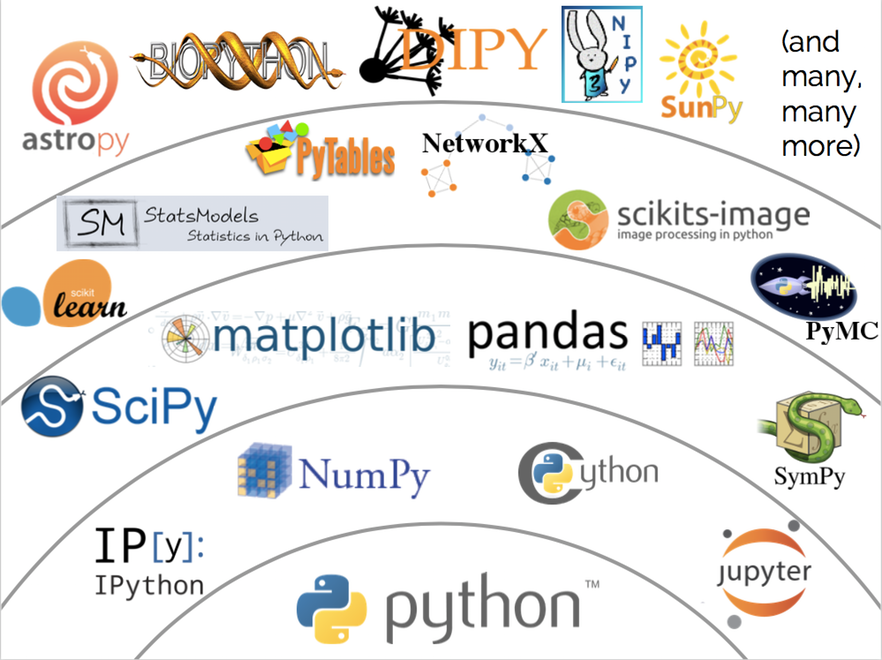
\includegraphics[width=8.8cm]{images/python_ecosystem.png}
	\end{figure}
	
	\blfootnote{\scriptsize https://www.datacamp.com/community/blog/python-scientific-computing-case}
	
\end{frame}



% PREGUNTAS
\begin{frame}

	\frametitle{¿Dudas? ¿Preguntas?}
	
	\begin{figure}
		% https://pixabay.com/en/airplane-takeoff-plane-2745898/
		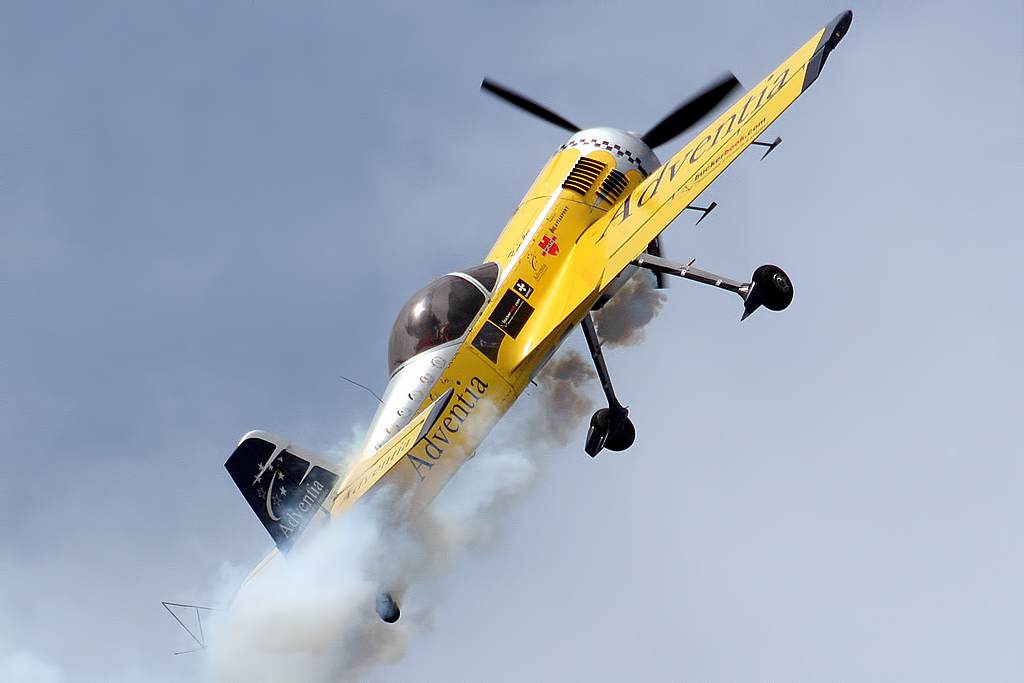
\includegraphics[width=8cm]{images/Sukhoi_Su-31_Ramon_Alonso_EC-HGL.jpg}
	\end{figure}

	\begin{center}
		\Large ¡Gracias por asistir!
	\end{center}
	
\end{frame}

	
\end{document}